\documentclass[addpoints]{exam}

% Header and footer.
\pagestyle{headandfoot}
\runningheadrule
\runningfootrule
\runningheader{CS 113 Discrete Mathematics}{HW I: Sets}{Spring 2020}
\runningfooter{}{Page \thepage\ of \numpages}{}
\firstpageheader{}{}{}
\usepackage{graphicx}
% \qformat{{\large\bf \thequestion. \thequestiontitle}\hfill[\totalpoints\ points]}
\boxedpoints
\printanswers

\title{Homework I: Sets\\ CS 113 Discrete Mathematics\\ Habib University -- Spring 2020}
\author{mb05987}  % replace with your ID, e.g. oy02945
\date{29 January 2020}

\begin{document}
\maketitle

\begin{questions}


  \question[5]
  Write down $\mathcal{P}(X)$ if 
  $ X = \{ \emptyset, \{\alpha, \beta, \gamma \}, \gamma, \{\{ \alpha, \beta \} \} \}$.
  \begin{solution}
  \
    $\mathcal{P}(X) = \{\emptyset, \{\emptyset\},$
   $ \{\{\alpha, \beta, \gamma\}\},$
   $\{\gamma\},$
   $ \{\{\{\alpha, \beta \}\}\}, $
   $ \{\emptyset, \{\alpha,\beta,\gamma\}\},$
   $ \{\emptyset,\gamma\},$
   $\{\emptyset,\{\{\alpha,\beta\}\}\},$
   
   $ \{\{\alpha, \beta, \gamma\},\gamma\},$
    $\{\{\alpha,\beta,\gamma\},\{\{\alpha,\beta\}\}\},$
   $ \{\gamma,\{\{\alpha,\beta\}\}\},$
    $\{\emptyset,\{\alpha,\beta,\gamma\},\gamma\},$
    
   $ \{\emptyset,\{\alpha,\beta,\gamma\}, \{\{\alpha,\beta\}\}\},$
   $ \{\emptyset,\gamma, \{\{\alpha, \beta\}\}\},$
    $\{\{\alpha,\beta,\gamma\},\gamma,\{\{\alpha,\beta\}\}\},$
   $ \{ \emptyset, \{\alpha, \beta, \gamma \}, \gamma, \{\{ \alpha, \beta \} \} \}\}$

  \end{solution}
  \question
  \begin{parts}
    \part[5] 
    Assume that RO has asked for your help to generate a set that contains all the possible pairs of DSSE faculty and DSSE courses at Habib University. Describe the sets and set operations that you can use to provide RO the desired set.
    \begin{solution}
     The set operation would be "Cartesian Product" as it is a set of all ordered pairs.The pair is written as: \{(a,b)\} where a is an element of DSSE faculty and b is an element of DSSE courses.
     
    \end{solution}

    \part[5] Imagine that the the operation above is extended to include an additional set that contains all the time slots when a course can be scheduled. Explain the outcome of the obtained set.
    \begin{solution}
      Let A be the set of the DSSE faculty and B be the set of  the DSSE courses.
      
      A x B = \{(a,b)\} if we add another set of time slots where C represents set of the time slots. Then 
      
      (A x B) x C = \{((a,b),c)\} then the Cartesian product would have three ordered pairs. 
    \end{solution}
  \end{parts}
  
  \question
      let x $\in$  $\overline{ A \cup \overline{B}}$

      ${\overline{A} \cap {B}} $.

  The \textit{symmetric difference} of two sets $A$ and $B$ is defined as $A\oplus B = (A-B) \cup (B-A)$. It is also known as the \textit{disjunctive union} as it contains all those elements which are in either of those sets, but not in their intersection. 
  \begin{parts}
    \part[5] Prove that $A\oplus B = (A \cup B)-(A \cap B).$
    \begin{solution}
     $(A \cup B)-(A \cap B) = (A-B) \cup (B-A) $
     
     Taking the left hand side:
         
    $(A \cup B)-(A \cap B)$
        
    1)Set difference: A-B = A $\cap \overline$ B
    
    let A = $(A \cup B)$ and B = $(A \cap B)$
    
    Then $(A \cup B) \cap \overline{(A \cap B)}$
    
    2) De Morgan's law: $\overline{(A \cap B)}$ = $\overline A$  $\cup$ $\overline B$
    
    Then, $(A \cup B) \cap (\overline A \cup \overline B)$
    
    3) Distributive law:
        $A \cup (B \cap C)$ = $(A \cup B) \cap (A \cup C)$
        
        $A \cap (B \cup C)$ = $(A \cap B) \cup (A \cap C)$
    
Then,$((A \cup B) \cap \overline A) \cup (( A \cup B) \cap \overline B)$
      
Again we will apply distributive law:
$((A \cap \overline A) \cup (B \cap \overline A)) \cup ((A \cap \overline B) \cup (B \cap \overline B))$ 

Now complement law: $A \cap \overline A = \emptyset$

And Identity law:$A \cup \emptyset = A$

$((\emptyset) \cup ( B \cap \overline A)) \cup ((A \cap \overline B) \cup (\emptyset))$

$(B - A) \cup (A-B)$
Proved Right hand side
      
      
      
    \end{solution}

    \part[10] For three sets $A, B,$ and $C$ we define the symmetric difference as $A\oplus B\oplus C = (A\oplus B)\oplus C $, meaning using the definition twice. Draw the Venn diagram of this set and express it as in part (a).
    \begin{solution}
    \begin{center}
    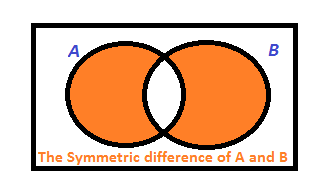
\includegraphics[width=5cm]{venn1.png}
    This figure shows the $A \oplus B$ where the intersection part is empty.
    
    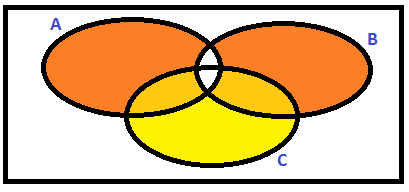
\includegraphics[width=5cm]{Venn2.png}
   In figure 2, when set C joins the resultant set of $A \oplus B$.
   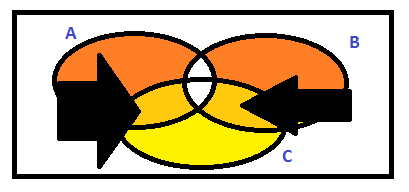
\includegraphics[width=5cm]{Venn3.png}
   In figure 3, The common part (shown by arrow) would be subtracted/excluded.
   
   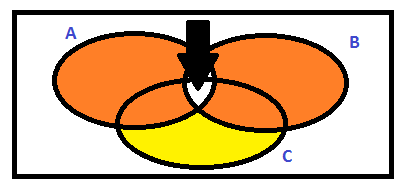
\includegraphics[width=5cm]{Venn4.png}
   Whereas Over here (shown by arrow) is not common therefore this part and rest A,B,C part are taken Union while the common part are taken out.
   
    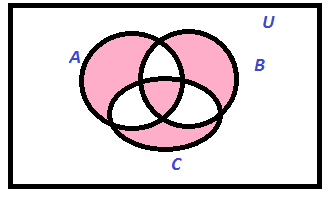
\includegraphics[width=5cm]{venn.png}
    This is the final set we get of (A\oplus B)\oplus C $
    \end{center}
    \end{solution}
  \end{parts}

  \question
  Let $A$ be the set of all numbers that are divisible by 6 and $B$ the set of all numbers that are divisible by $10$.

  \begin{parts}
    \part[5] Write the sets $A$ and $B$ in proper set notation and describe $A \cap B$ as simply as possible.
    
    \begin{solution}
      $ A =\{x\set |x \in Z \wedge x \div 6 = = 0\}$
      
      $ B = \{x\set |x \in Z \wedge x \div 10 = = 0\}$
      
      $ A \cap B = \{x \set | x \in A \wedge x \in B\}$ 
      
       $A \cap B$ is representing all the possible elements that are in both set A and set B.
      
    \end{solution}
    
    \part[5] What is $A \oplus B$? Describe it using set notation and prove that it is indeed the symmetric difference of $A$ and $B$.
    \begin{solution}
     As $A \oplus B$= $( A- B) \cup (B-A)$ = $( A \cup B) - ( A \cap B)$ is proved in Q3 part (a) which defines as elements are either found in A or in B but not in both.
          $A\oplus B$ by above definition the set notation would be :
      
        $A \oplus B =\{x\set|x \in A \vee x \in B \} \wedge \neg \{x\set | x \in A \wedge x \in B \}$
        
         by definition union would be:
         
       $A \oplus B =\{x\set|x \in A \cup B \} \wedge \neg \{x\set | x \in A \wedge x \in B \}$
       
        Whereas Intersection is:
       
        $A \oplus B =\{x\set|x \in A \cup B \} \wedge \neg \{x\set | x \in A \cap B \}$
        
        And the difference:
        
        $A \oplus B =\{x\set|x \in A \cup B -  A \cap B \}$
        = $(A \cup B)-(A \cap B)$
    \end{solution}

    \part[5] List down the elements of $A$, $B$, and $A \oplus B$ if $U = \{x\in \mathcal{N} \mid x \leq 60 \}$.
    \begin{solution}
      $A = \{ 6,12,18,24,30,36,42,48,54,60\}$
      $B = \{ 10,20,30,40,50,60\}$
      
      $ A\oplus B$ = $\{ 6,10,12,18,20,24,36,40,42,48,50,54\}$
    \end{solution}
  \end{parts}

  \question
  Show that $\overline{ A \cup \overline{B}} = \overline{A} \cap B$.
  \begin{parts}
    
    \part[5] by using set identities.
    \begin{solution}
    Left hand Side:
    
    According to De Morgan's Law:  $\overline{ A \cup {B}} = {\overline{A} \cap \overline{B}}$
    
     so the $\overline{ A \cup \overline{B}}$ can be represented as
      ${\overline{A} \cap \overline \overline{B}}$
      
      The double complement of B is  B itself therefore we will get 
      
      ${\overline{A} \cap {B}} $ which is equal to Right hand side.
     
    \end{solution}
    
    \part[5] by proving that each set is a subset of the other.
    \begin{solution}
      $\overline{ A \cup \overline{B}} \subset  \overline{A} \cap B$
      
      Left Hand Side:                   
      let x $\in$  $\overline{ A \cup \overline{B}}$
      
      Then x $\notin$ $( A \cup \overline{B}})$ 
      
      That is, $\neg$ $(x \in A \vee x \in \overline{B}})$ 
      
      Then x $\notin$ A $\wedge$ x $\notin \overline{B}$
      
      That is, x $\in \overline $ A $\wedge$ x $\in \overline \overline$ B
      
      That is, x $\in \overline $ A $\wedge$ x $\in$ B
      
      which is, x $\in \overline{A} \cap B$
      
     Right hand side:
     
       Now, let $ x \in \overline{A} \cap B$ \\
      Then, $x \in \overline{A}$ $\wedge$ $ x \in B$\\
      Then, $x \notin A$ $\wedge$ $ x \notin \overline{B}$\\
      Then, $x \notin A \cup \overline{B}$\\
      So, $x \in \overline{(A \cup \overline{B})}$\\
      Hence, we Have Proved That: $  (\overline{A} \cap B) \subset (\overline{A \cup \overline{B}})$
      \end{solution}
    
  \end{parts}
    



\end{document}
